% Preamble
\documentclass[12pt]{article}

% Packages
\usepackage[left=3.0cm, right=1.5cm, top=2.0cm, bottom=2.0cm]{geometry}

\usepackage[utf8]{inputenc}
\usepackage[T2A]{fontenc}
\usepackage[russian]{babel}
\usepackage{amsmath, amsfonts, amssymb}
\usepackage{graphicx}
\usepackage{wrapfig}
\usepackage{fancyhdr}
\usepackage[shortlabels]{enumitem}
\usepackage{svg}
\usepackage{amstex}
\usepackage{colortbl}
\usepackage{bm}

\renewcommand{\vec}{\textbf}
\newcommand{\cross}{\times}

\pagestyle{fancy}
\fancyhead[L]{Работа №0.0.0}
\fancyhead[R]{Белинский Т.Д.\quad Б05-206}

% Document
\begin{document}
    \section*{0.0.0. НАЗВАНИЕ}
    \ \par
    \textbf{Цель работы:} бла

    \textbf{Оборудование:} бла бла

    \subsection*{Теоретическая часть}
    \ \par


    \subsection*{Экспериментальная установка}
    \ \par


    \begin{figure}[h]
        \centering
        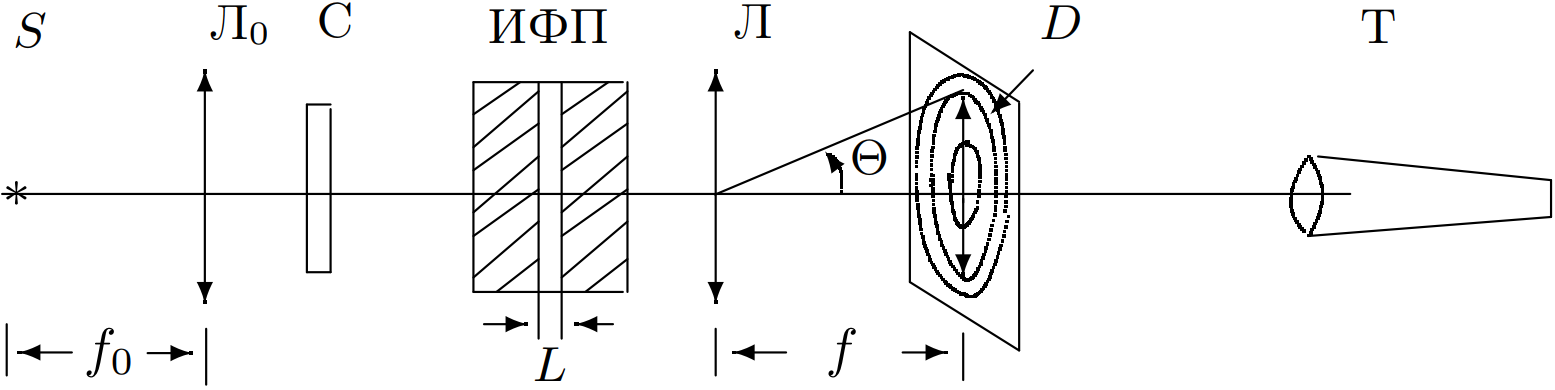
\includegraphics[width=\linewidth]{pic/setup}
        \caption{}
        \label{fig:fig1}
    \end{figure}



    \subsection*{Результаты и обработка}
    \begin{enumerate}
        \item
    \end{enumerate}

    \subsection*{Выводы}
    \begin{itemize}
        \item
    \end{itemize}
\end{document}